\documentclass[11pt,a4paper]{scrbook}
\usepackage{geometry}	
\usepackage[utf8]{inputenc}
\usepackage[T1]{fontenc}
\usepackage[pdftex]{graphicx}
\usepackage[ngerman, english]{babel} % the language specified at the end of the list will be used !!
\usepackage{colortbl}	
\usepackage{soul}
% For APA referencing style
\usepackage{apacite}
\renewcommand{\familydefault}{\sfdefault}
\usepackage{xcolor}
\definecolor{uhhred}{cmyk}{0,100,100,0}
\usepackage{float}
\usepackage[ddmmyyyy]{datetime}
\usepackage{comment}
\usepackage[acronym,nomain]{glossaries}

 
% Generate the glossary
\makeglossaries
 
%%%%%%%%%%%%%%%%%%%%%%%%%%%%%%%%%%%%%%%%%%%%%%%%%

\newacronym{ER}{ER}{Emotion Recognition}
\newacronym{EEG}{EEG}{Electroencephalography}
\newacronym{ADR}{ADR}{Action Design Research}

%%%%%%%%%%%%%%%%%%%%%%%%%%%%%%%%%%%%%%%%%%%%%%%%%%

\begin{document}

\frontmatter  % The \frontmatter declaration makes the pages numbered in lowercase roman
\newgeometry{centering,left=2cm,right=2cm,top=2cm,bottom=2cm}
\begin{titlepage}

\includegraphics[scale=0.3]{UHH-Logo_2010_Farbe_CMYK.pdf}
\vspace*{2.0cm}
\Large
\begin{center}
{\color{uhhred}\textbf{\so{MASTER THESIS}}}
\vspace*{1.0cm}\\
{\textbf{at the University of Hamburg in the Department of Computer Science in the master's programme IT Management and Consulting}}
\vspace*{2.0cm}\\
{\LARGE \textbf{Title:}}
\vspace*{0.4cm}\\
{\LARGE Visual Emotion Recognition In-The-Wild}
%{\LARGE Visual Emotion Recognition In-The-Wild: Prediction of Valence/Arousal and Assessment of Application scenarios}
%{\LARGE Identifying customer intentions in real-time video consultations through emotion recognition: Analysis of viability and value co-creation by implementation of a prototype}
\vspace*{1.5cm}\\
presented by
\vspace*{0.4cm}\\
Tobias Kick
\end{center}
\vspace*{2.0cm}

\noindent
MIN-Faculty \vspace*{0.25cm} \\
Department of Computer Science\vspace*{0.25cm} \\
Program: IT Management and Consulting\vspace*{0.25cm} \\
Research group: Computer Vision\vspace*{0.25cm} \\
Matriculation number: 7213712 \vspace*{0.5cm} \\
%Submission date: 15/12/2020 \vspace*{0.5cm} \\  
Supervisor: Noha Sarhan \vspace*{0.25cm} \\
First assessor: Prof. Dr. Simone Frintrop \vspace*{0.25cm} \\
Second assessor: Prof. Dr. Tilo Böhmann

\end{titlepage}

\restoregeometry

%%%%%%%%%%%%%%%%%%%%%%%%%%%%%%%%%%%%%%%%%%%%%%%%%%%%%%%%%%%%


\chapter{Abstract}
Here is the abstract

%%%%%%%%%%%%%%%%%%%%%%%%%%%%%%%%%%%%%%%%%%%%%%%%%%%%%%%%%%%%

\tableofcontents

\printglossary

%%%%%%%%%%%%%%%%%%%%%%%%%%%%%%%%%%%%%%%%%%%%%%%%%%%%%%%%%%%%
%%%%%%%%%%%%%%%%%%%%%%%%%%%%%%%%%%%%%%%%%%%%%%%%%%%%%%%%%%%%
\mainmatter
\chapter{Introduction}
%% (topic; problem with current research where is the flow; how do I suggest to make it different; goal; which dataset; what will the contribution be)


%%%%%%%%%%%%%%%%
{\LARGE Collection of literature} 
\newline
Paper in 2007 used a two stream architecture, from acoustic features, as well as the semantics of the conversation. They could prove that it is significant for Call-Center data to have semantics associated and deliver better results than just the use of acoustic features. \cite{Gupta:2007:Two-StreamER}
\newline




%%%%%%%%%%%%%%%%%%%%%%%%%%%%%%%%%%%%%%%%%%%%%%%%%%%%%

\chapter{Related Work}
% (backing up what I claimed in the introduction; what have other people done?; Inspired by other areas of research; what was good in those papers and where are the weakpoints)




Even though a lot of big companies, like Google or IBM, use and sell emotion recognition technologies, a review of psychological research argues that the belief of reliably corresponding facial expressions with emotions is unfounded. \cite{Vincent:2019:EmotionRecCantBeTrusted}

\section{Emotion Recognition}
Maybe here also mention the state of:
- Facial recognition + bounding boxing with MTCNN \cite{Zhang:2016:MTCCN}
approach: tasks of face detection, bounding boxing and landmark detection are closely related and somehow dependent on each other. Thus they made use of a three layered CNN architecture where they start to detect faces in the first CNN, go over to set the bounding box and then detect the facial landmarks. All this combined in one three-layered architecture, namely MTCNN - Multi-Task Convolutional Neural Network
This approach delivered significantly better results over multiple state-of-the-art architecture for face detection, alignment and landmark detection from the year 2016.
- Emotion recognition from faces (Model + Landmark)
- Landmark detection separate?
\newline\newline
Classification/representation of emotions:
- discrete emotion classes (usually 6)
- 2D Space Model \cite{Hupont:2010:FacialEmotionsIn2DAffectiveSpace}
- 3D Space Model \cite{Verma:2017:3D-VAD}
\newline\newline
This classification approach is still widely used in \gls{ER} research today, next to another approach called Continuous Affective Space. In 2010, the authors \citeauthor{Hupont:2010:FacialEmotionsIn2DAffectiveSpace} \cite{Hupont:2010:FacialEmotionsIn2DAffectiveSpace} came up with a way of measuring emotions as a psychological 2-dimensional continuous affective space. Through mapping emotions into a 2D space they are able to consider intermediate emotional states. In practice, this means, that instead of categorizing emotions, like 'happy' and 'angry', emotions are represented by two variables in a 2-dimensional space.
\newline\newline
The trend in research on \gls{ER} during the last years was strongly defined by the challenge of fusing multiple input signals for better prediction results. Most scientific contributions in this area, like the papers \cite{Yan:2016:MultiClueFusion} and \cite{Hossain:2019:AudioVisualER}, were fusing audio with visual signals in order to improve their \gls{ER}. Another paper \cite{Xing:2019:EEGAudioVisual} made use of combining EEG with audio and visual signals. However, the possibilities are not restricted to those mentioned input signals. As the authors in a summary on Speech Emotion Recognition (SER) \cite{Akcay:2020:SpeechEmotionRecognition(SER)} point out, audio signals could be combined with visual signals, physiological signals, linguistic features, mouse movements and keystroke dynamics.
\newline\newline
In 2016: Made use of multi clue fusion to further enhance the accuracy of an emotion recognition in the Wild. They showed that with using only the VGGFace model as a predictor for the Emotion Recognition challenge, they got a surprisingly high accuracy of about 36 per cent. They also mention that it the model will perform better as they recognize emotions over multiple frames and conduct fine-tuning on the VGGFace model. (Fintuning = the adaption of a pre-trained model to the current challenge, usually done together with a new dataset)\cite{Yan:2016:MultiClueFusion}
\newline\newline
Furthermore, they detect faces with Single Shot Detector (SSD) and whenever it fails, they crop the image manually so far, that the detector "has" to detect it. However, in the approach describe in this thesis, images with a non-detectable face will be passed into the model in their original size. Thus, no manual cropping is being conducted. Additionally, they focus on the concept of action units (AU) together with landmarks. They define a facial expression is a combination of several action units (AU) movements, with the action units being the trajectories of vital facial
landmarks.\cite{Yan:2016:MultiClueFusion}


\section{Human intention identification}
Current literature about the identification of human intentions through Emotion Recognition is very sparse. The research done in this area is mostly about detecting customer satisfaction. The authors in the paper "Measuring Customer Satisfaction through Speech using Valence-Arousal Approach" \cite{Kamaruddin:2016:MeasuringCustomerSatisfaction} could infer customer satisfaction with a very simple approach, while still lacking accuracy. Another example is a Master thesis from 2018, where the author \cite{Esser:2018:LandmarkDetection} managed to visualize the pain experience of patients in a hospital through the use of \gls{ER}. Even though there is currently no literature that exactly matches this field, another study conducted in 2012 \cite{Dong:2012:UnderstandHumanImplicitIntention}, was able to infer human intentions, in this experiment by agreeing or disagreeing toward a statement. However, they were only able to do this by subjecting their test persons to an \gls{EEG} analysis.
\newline\newline
Recognized emotions and used them to calculate a level of interest L, which is calculated as follows: L = W x I. Where I stands for the intensity of an emotion and is calculated through summing up all values from valence, arousal and stance (in a 3D affect space) and mapping these to a range of -5 to +5.
The weight W is represented by a number in the range of 0 to +1 and measures the relative number of images in a sequence that concentrate most of a motion. The lower the number, the closer the coefficient to 1.\cite{Yeasin:2006:MeasurmentOfInterestFromVideo}
\newline\newline
Paper from 2012 used customer words and comments to detect customer satisfaction through Emotion Recognition in this information:
\begin{quote}
    Using an annotated emotion corpus (Ren-CECps), we
    first present a general evaluation of customer satisfaction
    by comparing the linguistic characteristics of emotional
    expressions of positive and negative attitudes. The associations in four negative emotions are further investigated.
    After that, we build a fine-grained emotion recognition
    system based on machine learning algorithms for measuring customer satisfaction; it can detect and recognize
    multiple emotions using customers’ words or comments.
    The results indicate that blended emotion recognition is
    able to gain rich feedback data from customers, which can
    provide more appropriate follow-up for customer relationship management.\cite{Ren:2012:ERforCustomerSatisfaction}
\end{quote}

In another paper from 2016 \cite{Kamaruddin:2016:CustomerSatisfactionFromVA} the author build upon the hypothesis that the customer is satisfied if he/she is experiencing happiness and neutral emotion whereas if he/she is experiencing sadness or anger, the customer is dissatisfied. They were using Valence and Arousal values and split them up into four emotional values, including one for neutral emotion. They made use of a threshold to define the neutral emotion class. From these classes they directly inferred whether the customer was satisfied or not. Their accuracy stems from the correct prediction of this classes and is with 39 percent accuracy much better than random guessing with 25 percent.

\begin{quote}
    We hypothesize that if the valence value is positive (happiness and calm), the customer is satisfied whereas if the valence value is negative (anger and sadness), the customer is not satisfied. Although such approach is simple, it may give us the better understanding of neutral region threshold so that it can be further used for analysis. \cite{Kamaruddin:2016:CustomerSatisfactionFromVA}
\end{quote}

\begin{figure}[H]
  \begin{center}
  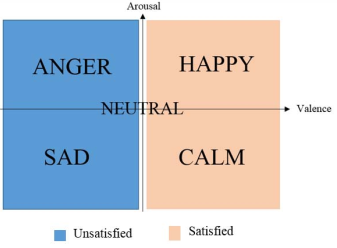
\includegraphics[angle=0, width=0.6\textwidth]{Figures/Satisfaction_from_VA.PNG}
  \caption{Satisfaction inference from VA values}
  \label{fig:SatisfactionFromVA}
  \end{center}
\end{figure}

The FaceReader product of the company Noldus\cite{Noldus:2020:Facereader} makes use of the seven basic emotions ,like happy or angry, and convert them into values for valence and arousal.

In a survey conducted in 2006 \cite{Poirier:2016:AdsFacialExpression}, the authors measured the effectiveness of ads through facial expressions.
\begin{quote}
    emotional journey, which relates to the positive or negative emotional variation  (valence between -1 and 1 where -1: 100\% negative expression, 1: 100\% positive expression and 0: neutral expression), remains the most powerful predictor of ad appreciation 
\end{quote}

\section{Value Co-Creation}
The co-creation of value is a core concept inside the Service-Dominant Logic (S-D Logic) that every client interaction can be described as a service. In this logic, the service's value is co-created by experiences between the service provider and the service user.\cite{Payne:2008:ValueCo-Creation}
\newline\newline
In comparison to S-D Logic where value is embedded in experiences, in the 'traditional' Goods-Dominant Logic (G-D Logic) value is embedded in goods and thus is only created by the produce of goods, but not by the user/client. \cite{Payne:2008:ValueCo-Creation}
\newline\newline
As a result, S-D Logic places the client at the same level of companies as the co-creator of value. As both of them engage in dialog through the product design and delivery stage, thus co-creating value through customized products. This co-creation can take place, for example, through the emotional engagement of the customer, as well as the co-design of product or even the transfer of labor to the customer (e.g. IKEA products). \cite{Payne:2008:ValueCo-Creation}
\newline\newline
\textbf{How does value co-creation manifest itself in this thesis?}
\chapter{Methodology}
% (diagram: data flow ; from input to output, everything in between; a paragraph on each module)
\section{Research paradigm: Action-Design-Research} 
As all of these items are conducted in a very agile approach, namely with \gls{ADR}, it is assumed that evaluation of tasks will take place immediately before each task was completed. There will be a strong focus on interviews and a constant exchange with experts. 

%%% 

\section{Development technique: Minimum Viable Product (MVP)}
The concept of a Minimum Viable Product (MVP) was first introduced by \citeauthor{Ries:2011:TheLeanStartUp} E. in \citeyear{Ries:2011:TheLeanStartUp} as a methodology for creating a 'Lean StartUp'. It aims at starting the learning process as early as possible through integrating early adopter's feedback.\cite{Lenarduzzi:2016:MVP}
\newline\newline
The Build-Measure-Learn loop is one of the core principles in 'Lean StartUp' which allows entrepreneurs to learn whether to give up or persevere with a current build \cite{Lenarduzzi:2016:MVP}. This build is usually defined as a MVP. The author \citeauthor{Ries:2011:TheLeanStartUp} E. describes an Minimum Viable Product as follows:
\begin{quote}
    "The MVP is that version of the product that enables a full turn of the Build-Measure-Learn loop with a minimum amount of effort and the least amount of development time."\cite{Ries:2011:TheLeanStartUp}
\end{quote}
However, a MVP is still far from being complete, on the contrary, it requires additional effort during building as its outcomes will be presented to potential customers and its feedback needs to be measurable. \cite{Ries:2011:TheLeanStartUp}
\newline\newline

\textbf{Paragraph -> How does MVP manifest itself in this thesis?}

    
    
%%%%%%%%%%%%%%%%%%%%%%%%%%%%%%%%%%%%%%%%%%%%%%%%%%%%%


\section{Methods}	
\begin{figure}[H]
  \begin{center}
  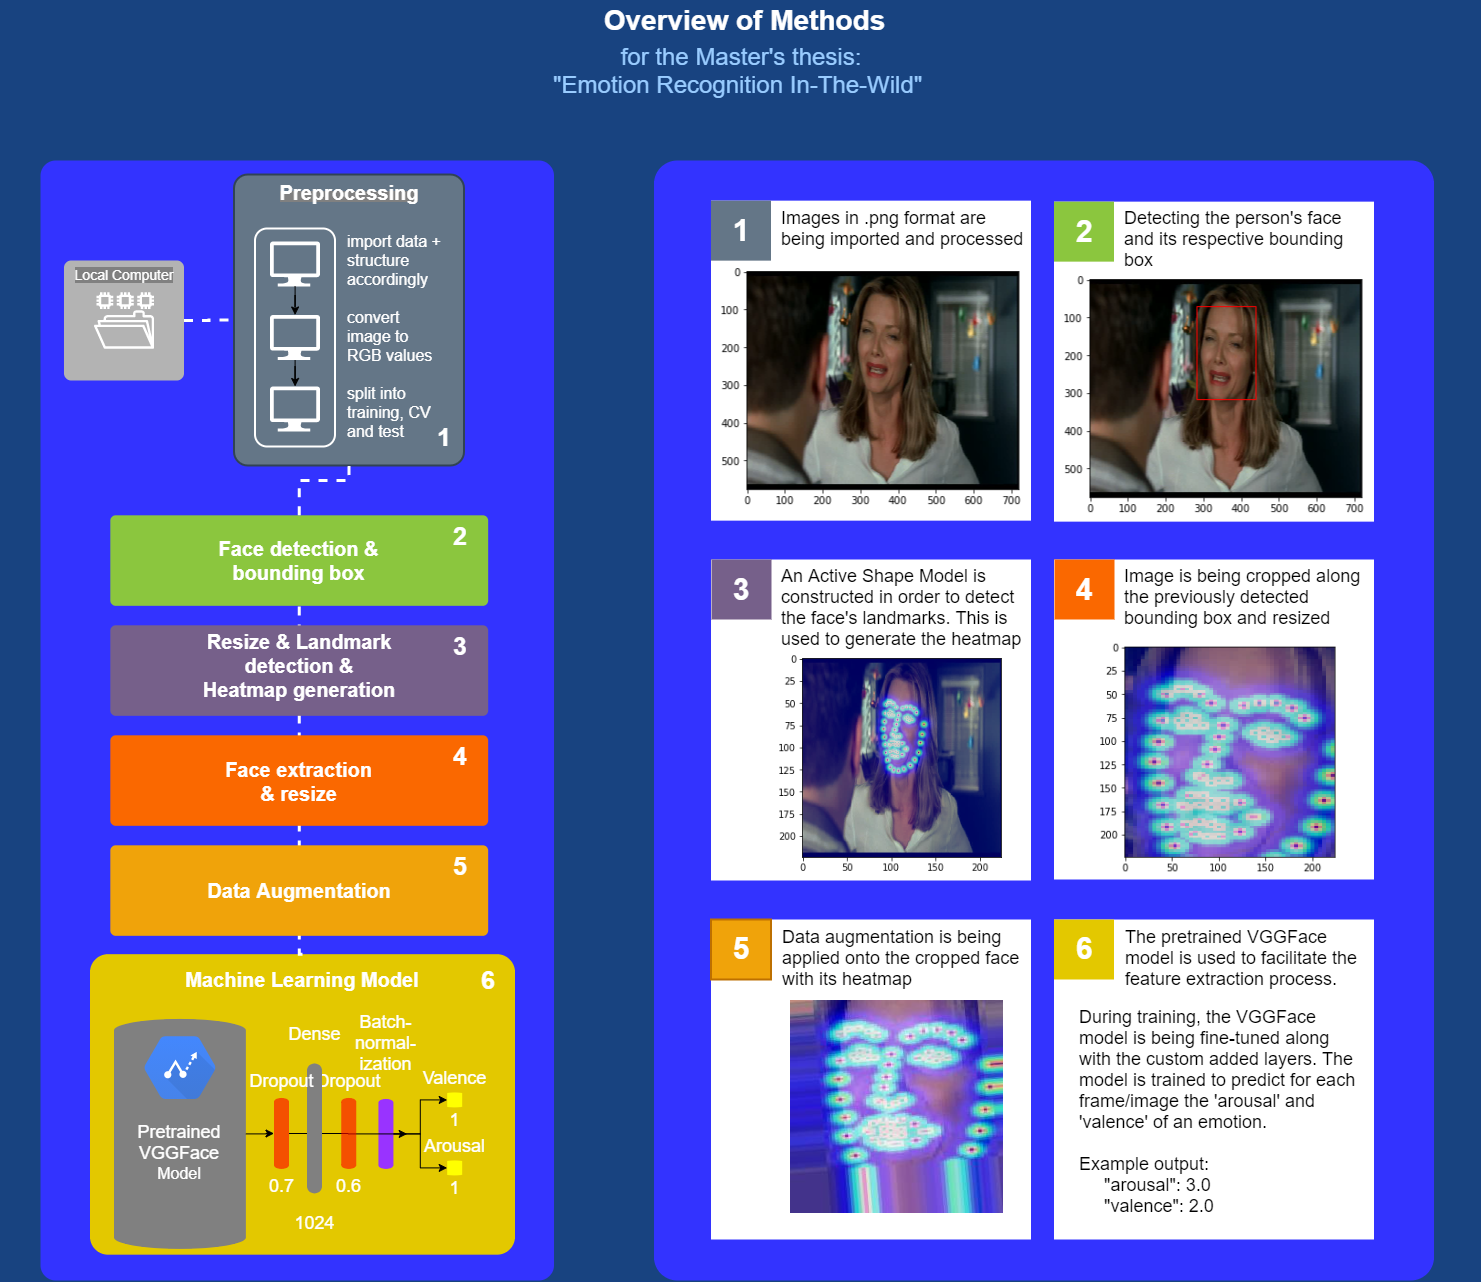
\includegraphics[angle=90, width=1.0\textwidth]{Figures/DataFlow_Diagram.png}
  \caption{Overview: Machine Learning Model - Components}
  \label{fig:MachineLearningModelComponents}
  \end{center}
\end{figure}

Approach:
1. Face detection
using MTCNN (Simultaneous face detection, face alignment, bounding boxing and landmark detection)\cite{Brownlee:2019:VggFace2HowToFaceRec}

2. Highlighting faces
draw the bounding box in an image and plot it\cite{Brownlee:2019:VggFace2HowToFaceRec}

3. Face extraction
extracting the face according to the identified bounding box
\cite{Brownlee:2019:VggFace2HowToFaceRec}

4. Face recognition
Using the VGGFace pretrained Resnet50 model to recognize emotions (training + prediction)
\cite{Sharma:2018:RealTimeFacialExpression}


\subsection{Preprocessing}
\subsubsection{Data construction}
Firstly, before reading in the actual image data, data description files are being read and analyzed. These description files are located inside subfolders of the dataset, one file for each speaker.
After all these description files are being read in from the data structure, a list of all image-filenames and their respective labels for valence and arousal is created.
\newline\newline
These lists are then being shuffled for a better randomization and are then split into training and testing data. Hereby, 25 per cent of the part of the dataset that is read in (a small part is reserved for final prediction testing) is used as a validation set.
\newline\newline
Furhtermore, labels are preprocessed by splitting each value through the number 5, as the original data, which ranges from -5 to 5, needs to be resized to a range of -1 to 1 in order to fit the activation function of the final layer which is a tanh activation function.
\newline\newline
The last preprocessing step involves loading all the images, converting it into RGB values and then extracting the face while using the face detection techniques described in the next chapter. The cropped output image will have a shape of 224x224x3 and will be permanently saved so that this step doesn't have to be repeated each time the model is being trained. Furthermore, the model can then reach back to this array of extracted images and directly use them to train or finetune the model.


\subsection{Face detection}
Made use of MTCCN to detect faces in images, set a bounding box and extract the face of an image.\cite{Zhang:2016:MTCCN}

1. Read the image, convert it to gray-scale and save it.
2. Read that gray-scale saved image, then detect face in it using HAAR cascade.
3. Crop the image to the detected face and resize it to 350*350 and save the image.
4. Read that processed cropped-resized image, then reshape it and normalize it.
5. Then feed that image to VGG-16 and create bottleneck features of that image and then reshape it.
6. Then use our own model for final prediction of expression.\cite{Sharma:2018:RealTimeFacialExpression}

\subsection{Finetuning VGGFace}

1. Pretrained VGGFace Model
—In this paper, we introduce a new large-scale face dataset named VGGFace2. The dataset contains 3.31 million images of 9131 subjects, with an average of 362.6 images for each subject. Images are downloaded from Google Image Search and have large variations in pose, age, illumination, ethnicity and profession (e.g. actors, athletes, politicians). 
The dataset was collected with three goals in mind: (i) to have both a large number of identities and also a large number of images for each identity; (ii) to cover a large range of pose, age and ethnicity; and (iii) to minimise the label noise. We describe how the dataset was collected, in particular the automated and manual filtering stages to ensure a high accuracy for the images of each identity. To assess face recognition performance using the new dataset, we train ResNet-50 (with and without Squeeze-andExcitation blocks) Convolutional Neural Networks on VGGFace2, on MS-Celeb-1M, and on their union, and show that training on VGGFace2 leads to improved recognition performance over pose and age. Finally, using the models trained on these datasets, we demonstrate state-of-the-art performance on the face recognition of IJB datasets, exceeding the previous state-of-the-art by a large margin.\cite{Cao:2018:VGGFace2}
\newline\newline
The VGGFace model is at foremost used to extract features from the data and allow the custom built top layers to learn the connection between extracted features and desired output (=label). Additionally, it is also being finetuned, which means that is being adapted to the current challenge at hand. This is necessary because originally, the VGGFace model wasn't designed nor trained to be used for Emotion Recognition challenges. Hence, the layers inside the VGGFace model are being trained with the current dataset and their desired output labels. This is called finetuning, as the model will be adapted to better fit this Emotion Recognition challenge.
\chapter{Implementation}
% (more or less telling whats in my code; implementation details; describing dataset; which network and which hyper parameters do I use; how does the application look like)
\section{Setup}

Remote PC for Learning

Major frameworks and their respective versions:
Tensorflow:    tensorflow-gpu==1.14.0
               tensorboard==1.14.0
Keras: 2.3.1
Python: 3.6
MTCNN: 0.1.0
keras-vggface: 0.6


Command Line access:

Jupyter Notebook access to remote server:
For remoteuser@remotehost:
\begin{itemize}
    \item remoteuser@remotehost:
    jupyter notebook --no-browser --port=XXXX
    
    \item localuser@localhost:
    ssh -N -f -L localhost:YYYY:localhost:XXXX -L localhost:ZZZZ:localhost:WWWW remoteuser@remotehost
    (ZZZZ is port at local machine for the tensorboard, while WWWW represents the port on the remote machine on which tensorboard is running)
    
    \item localuser@localhost:
    http://localhost:YYYY
\end{itemize}
The jupyter notebook is being started up through running the 'localhost:YYYY' command in the web browser, while the tensorboard is started through the following command inside the jupyter notebook 'tensorboard --logdir <path> --port ZZZZ'

\section{Dataset}
Which dataset did I use for training and testing?
If AFEW-VA , then cite the paper and write sth. about it.
\cite{Kossaifi:2017:AFEW-VADatabase}
\cite{Dhall:2012:AFEWVA}
(two sources from README)

-> Structure of data
each video clips is split into multipe frames. All these frames are kept into one folder.
-> Structure of labels
Each folder with the respective frames for the video clip have a .json file named according the naming schema for the folders, e.g. folder name is '001' then the file for the labels will have the name '001.json'. This file contains for each frame a label/value for the emotional values of valence and arousal. Additionally it also includes the pre-labeled landmarks for face detection purposes. These landmarks are as of now (5th of July 2020) not utilized, as an external module is being used for the face detection task.

\begin{quote}
    To compare the performance of various features, we sampled regularly an equal number of frames from each sequence to obtain a set of frames representative of the whole dataset, which we then divided in 5 disjoint folds in a subject-independent manner (i.e. a subject does not appear in two different folds). We then performed a 5-fold cross-validation (i.e. we iteratively used one of the set for testing and the other 4 for training) to predict the valence and arousal values for each frame\cite{Kossaifi:2017:AFEW-VADatabase}
\end{quote}

\section{Architecture}

\begin{figure}[H]
  \begin{center}
  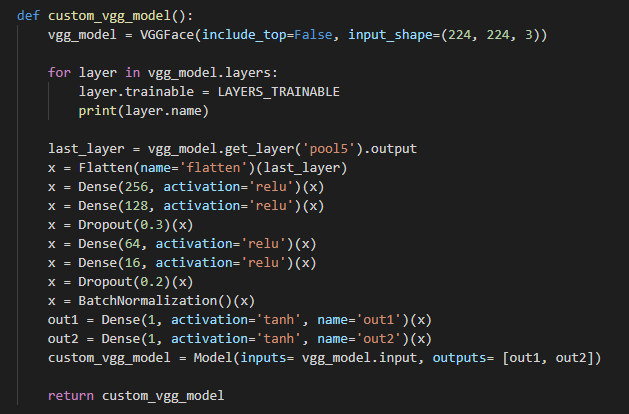
\includegraphics[angle=0, width=0.9\textwidth]{Figures/model_architecture.PNG}
  \caption{Architecture: Custom ML Model}
  \label{fig:ArchitectureCustomMLModel}
  \end{center}
\end{figure}

The model is using the X number of layers from the VGGFace model which layers can be either trained or not, depending on the purpose. The output of the last Pooling layer, after all the Convolutional layers, is being taken and used as an input into the custom built model.

The custom model consists firstly, of a Flatten layer bring the previous output in a fitting shape. Following this, there are 4 Dense layers with different numbers of parameters which decrease, so that information gets more and more crystallized towards the desired output. In between there are two Dropout layers and one BatchNormalization layer which are common techniques to prevent a ML Model from overfitting. Thus, using these techniques, the model can still perform well on a validation dataset.
\newline\newline
The output is split up into two variables which are defined by an Dense layer with activation 'tanh'. This split is necessary, because the metrics can then be applied to each of the outputs separately.
\newline\newline
Architecture strategy:
\begin{quote}
    The experiments in the paper 'Comparison of Fine-Tuning and Extension Strategies for Deep Convolutional Neural Networks' \cite{Pittaras:2017:FineTuningStrategiesComparison} show that the method of increasing the depth of a pre-trained network with one fully-connected layer and fine-tuning the rest of the layers on the target dataset can improve the network’s concept detection accuracy, compared to other fine-tuning approaches
\end{quote}


\section{Metrics}
The accuracy metric is a standard metric in Machine Learning, it tells you about the number of correctly predicted data points out of all data points. In a regression problem, like in this instance, it represents the percentage of how good the predicted values match the actual values.
\newline\newline
RMSE (Root-mean-squared error) and CORR (Pearson product-moment correlation coefficient) are the most commonly found metrics for Emotion Recognition challenges. 

\begin{quote}
    CORR gives information about the magnitude of the association, or correlation, as well as the direction of the relationship. \cite{2020:PearsonCorrelation}
\end{quote}

\begin{quote}
    Root Mean Square Error (RMSE) is the standard deviation of the residuals (prediction errors). Residuals are a measure of how far from the regression line data points are ... In other words, it tells you how concentrated the data is around the line of best fit. \cite{2020:RMSE}
\end{quote}

To sum it up, RMSE lets the observer grasp how exact the predicted value is, while CORR tells you how strong the relationship between prediction and label is.

\begin{figure}[H]
  \begin{center}
  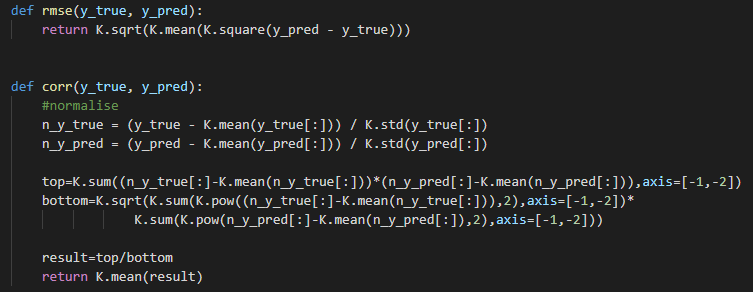
\includegraphics[angle=0, width=0.9\textwidth]{Figures/model_metrics.PNG}
  \caption{Model Custom Metrics}
  \label{fig:ModelCustomMetrics}
  \end{center}
\end{figure}

\section{Regularization}
This post covered a lot of topics, but hopefully you now have an idea of the basics of modeling, overfitting vs underfitting, bias vs variance, and model optimization with (cross-validation). \cite{Koehrsen:2018:OverfittingVSUnderfitting}

Prevention overfitting
https://elitedatascience.com/overfitting-in-machine-learning
\newline\newline
Another source:
Reducing overfitting through applying regularization to pretrained neural networks
https://sthalles.github.io/keras-regularizer/
\newline\newline
Callbacks: 
- Checkpoint for Best Model
- EarlyStopping
- Reduce Learning Rate on Plateau
- Lambda Calback: Setting the layers from the VGGFace model to trainable, for further fine-tuning, after a few epochs of training.

\begin{figure}[H]
  \begin{center}
  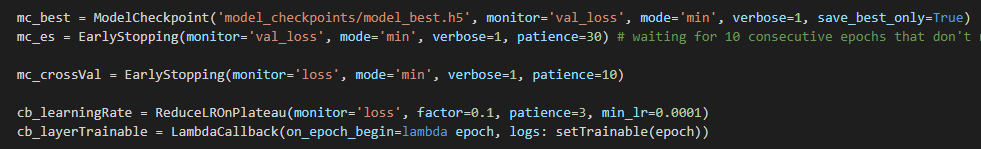
\includegraphics[angle=0, width=0.9\textwidth]{Figures/model_callbacks.PNG}
  \caption{Callbacks for the training process}
  \label{fig:CallbacksTraining}
  \end{center}
\end{figure}

When training I injected callbacks into the training function. These callbacks allow me to keep track of the best model and automatically saves this model according to a specified metric which is in this case the validation loss.\newline
Moreover, a second checkpoint, called 'EarlyStopping', is used to make the model step as soon as it is clear that no improvement is made and saves the last model. The early stopping checkpoint is waiting for 30 consecutive epochs during which a certain specified variable is not improving. In this instance, this checkpoint again is looking at the validation loss as the variable to be observed.

ReduceLearningRateOnPlateau = a checkpoint that automatically reduces the learning rate by a certain factor once it detects that a monitored variable is not improving for a certain period of epochs.

LambdaCallback is a custom callback function used in this case to execute a function on the beginning of each epoch. In this case, 


	
\chapter{Results and Analysis}
% (more tables and graphs; comparison; what other people achieved)
\section{Benchmark AFEW-VA Dataset}
Experiment on AFEW-VA dataset and results comparison along the metrics Accuracy, RMSE and CORR.
\newline
In the original paper from 2017, when the AFEW-VA database \cite{Kossaifi:2017:AFEW-VADatabase} was introduced, the author already provided a benchmark by comparing different methods, like SVR or DCNN, with the three metrics RMSE (Root Mean Squared Error), CORR (Correlation) and ICC (Interclass Correlation). 

\begin{table}[H]
\centering
\begin{tabular}{cc|ccc}
\multicolumn{1}{l}{} & \multicolumn{1}{l|}{\textbf{}} & \multicolumn{1}{l}{\cellcolor[HTML]{CBCEFB}\textbf{RMSE}} & \multicolumn{1}{l}{\cellcolor[HTML]{CBCEFB}\textbf{CORR}} & \multicolumn{1}{l}{\cellcolor[HTML]{CBCEFB}\textbf{ICC}} \\ \hline
FT-DCNN & \cellcolor[HTML]{F8FF00}\textbf{Valence} & 0.37 & 0.26 & - \\
(RGB images) & \cellcolor[HTML]{F8FF00}\textbf{Arousal} & 0.39 & 0.31 & - \\ \hline
MKL & \cellcolor[HTML]{F8FF00}\textbf{Valence} & 0.2639 & 0.401 & 0.274 \\
(Shape+DCT) & \cellcolor[HTML]{F8FF00}\textbf{Arousal} & 0.2229 & 0.445 & 0.34
\end{tabular}
\end{table}

The best performing method compared in this paper is the MKL (Multiple Kernel Learning) which performs best in comparison to other methods examined in this paper. In this method the authors utilized different kernels for each, shape features (Norm-shape) and appearance features (Hybrid-DCT).
\newline\newline
The FT-DCNN model, a fine tuned Deep Convolutional Neural Network follows a very similar approach as the one proposed here in this Master thesis. The model is trained on randomly sampled frames from video sequences (just like in this thesis). Fine tuning is being done with AlexNet, a pre trained model on the ImageNet dataset.
\newline\newline
The 'DeepDriver' paper \cite{Theagarajan:2018:DeepDriver} from the year 2018, used the AFEW-VA database to evaluate their approach. It consisted of taking multiple frames as a sequence and feeding them into either a CNN-only architecture or an CNN + LSTM architecture. Both methods heavily outperformed all benchmark results on the RMSE and CORR metric. The best result, using the CNN + LSTM, achieves the following results:


\begin{table}[H]
\centering
\begin{tabular}{c|cc}
\multicolumn{1}{l|}{\textbf{}} & \multicolumn{1}{l}{\cellcolor[HTML]{CBCEFB}\textbf{RMSE}} & \multicolumn{1}{l}{\cellcolor[HTML]{CBCEFB}\textbf{CORR}} \\ \hline
\cellcolor[HTML]{F8FF00}\textbf{Valence} & 0.093 & 0.639 \\ \hline
\cellcolor[HTML]{F8FF00}\textbf{Arousal} & 0.087 & 0.626 \\ 
\end{tabular}
\end{table}

These results were obtained by using a 3-fold cross validation approach for training and evaluation. However, the author made use of two different datasets, the AFEW-VA and MotorTrend's dataset. Due to the fact that the here implemented approach is only being trained on the AFEW-VA data, it cannot be objectively compared to results obtained through a training on two different datasets.
\newline\newline
A paper from 2020 \cite{Handrich:2020:SimultaneousPredVA} made use of cross-database validation for the recognition of valence and arousal in videos/images. They used the AFEW-VA database \cite{Kossaifi:2017:AFEW-VADatabase} as a validation dataset and achieved slightly better results for the CORR and ICC metrics. This shows that their approach is indeed an improvement to the 2017 benchmark paper. However, compared to the DeepDriver paper from 2018, the results are still lagging behind strongly. Their proposed CNN architecture is also based upon RGB images as an input and achieves the following results:

\begin{table}[H]
\centering
\begin{tabular}{cl|cc}
\multicolumn{1}{l}{} & \textbf{} & \multicolumn{1}{l}{\cellcolor[HTML]{CBCEFB}\textbf{RMSE}} & \multicolumn{1}{l}{\cellcolor[HTML]{CBCEFB}\textbf{CORR}} \\ \hline
\begin{tabular}[c]{@{}c@{}}AFEW-VA\\ database\end{tabular} & \multicolumn{1}{c|}{\cellcolor[HTML]{F8FF00}\textbf{Valence}} & 0.26 & 0.39 \\
only & \multicolumn{1}{c|}{\cellcolor[HTML]{F8FF00}\textbf{Arousal}} & 0.25 & 0.29 \\ \hline
\begin{tabular}[c]{@{}c@{}}Cross-\\ database\end{tabular} & \cellcolor[HTML]{F8FF00}\textbf{Valence} & 0.28 & 0.58 \\
validation & \cellcolor[HTML]{F8FF00}\textbf{Arousal} & 0.26 & 0.46
\end{tabular}
\end{table}

These results were obtained using 5-fold cross validation on the AFEW-VA database, while training on 70 percent and validating on 30 percent of the whole dataset. Thus, the results can be compared to the herein mentioned approach, but it leaves room for questions about which 30 percent of the data was used for testing and how it was shuffled.
\newline\newline
The results for the implemented model were achieved with the following training approach:\newline
At first, only the custom model is trained during 3 epochs with learning rate of 0.01, while the layers of the VGGFace model are frozen/non-trainable. After that, all layers inside the model are set to be trainable, including the layers of the VGGFace model. this is called fine-tuning. After 175 epochs of training with learning rate of 0.0001, the following results were produced:

\begin{table}[H]
\centering
\begin{tabular}{clll}
\multicolumn{1}{l}{\textbf{}} & \cellcolor[HTML]{9aff99}\textbf{ACC} & \cellcolor[HTML]{9aff99}\textbf{RMSE} & \cellcolor[HTML]{9aff99}\textbf{CORR} \\
\cellcolor[HTML]{F8FF00}\textbf{\begin{tabular}[c]{@{}c@{}}Valence\\ (out1)\end{tabular}} & 0.3499 & 0.1218 & 0.9509 \\ \hline
\cellcolor[HTML]{F8FF00}\textbf{\begin{tabular}[c]{@{}c@{}}Arousal\\ (out2)\end{tabular}} & 0.1807 & 0.1358 & 0.9341
\end{tabular}
\end{table}

This can also be seen in the following two graphs, the first representing the output for the 'Valence' and the second graph representing the 'Arousal'. Both graphs only show the results during the 175 epochs of training, while not displaying the initial three epochs.

\begin{figure}[H]
  \begin{center}
  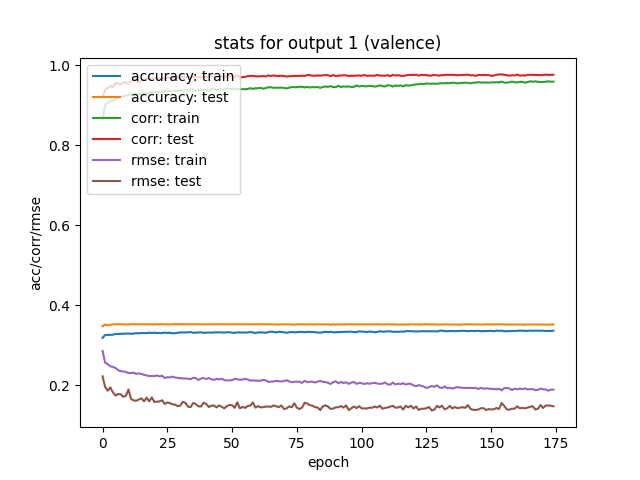
\includegraphics[angle=0, width=0.9\textwidth]{Figures/output1.png}
  \caption{Training progress for 'Valence'}
  \label{fig:TrainingProgressValence}
  \end{center}
\end{figure}

\begin{figure}[H]
  \begin{center}
  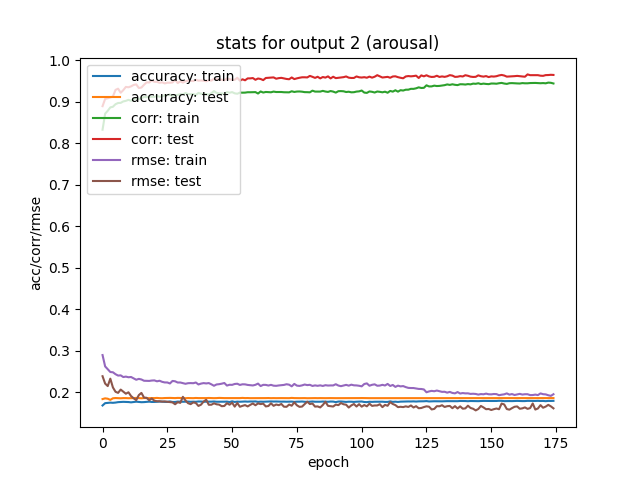
\includegraphics[angle=0, width=0.9\textwidth]{Figures/output2.png}
  \caption{Training progress for 'Arousal'}
  \label{fig:TrainingProgressArousal}
  \end{center}
\end{figure}

Even though these results are based on a 5-fold cross-validation, as done by two of the before mentioned papers, it is trained on completely shuffled data. Thus, training is not subject independent, which means, different frames from one specific person can appear in the training fold, as well as the testing fold. Implementing this, makes the training process harder and worse results are to be expected.
\newline\newline
The following table summarizes the results from a 5-fold cross-validation with subject-independent folds:
(Numbers can not be exactly specified, as they are being read from a chart)

\begin{table}[H]
\centering
\begin{tabular}{clll}
\multicolumn{1}{l}{\textbf{}} & \cellcolor[HTML]{9aff99}\textbf{ACC} & \cellcolor[HTML]{9aff99}\textbf{RMSE} & \cellcolor[HTML]{9aff99}\textbf{CORR} \\
\cellcolor[HTML]{F8FF00}\textbf{\begin{tabular}[c]{@{}c@{}}Valence\\ (out1)\end{tabular}} & 0.33 & 0.28 & 0.83 \\ \hline
\cellcolor[HTML]{F8FF00}\textbf{\begin{tabular}[c]{@{}c@{}}Arousal\\ (out2)\end{tabular}} & 0.18 & 0.26 & 0.80
\end{tabular}
\end{table}





\section{Results and comparison}
Comparing the above mentioned papers with the actual achieved results:

\begin{table}[H]
\begin{tabular}{clcc|cc}
\multicolumn{1}{l}{} & \multicolumn{1}{c}{\textbf{Architecture}} & \textbf{Evaluation} & \textbf{Metrics} & \multicolumn{1}{l}{\cellcolor[HTML]{9AFF99}\textbf{RMSE}} & \multicolumn{1}{l}{\cellcolor[HTML]{9AFF99}\textbf{CORR}} \\ \hline
\textbf{\begin{tabular}[c]{@{}c@{}}RESULTS\\ THESIS\end{tabular}} & \begin{tabular}[c]{@{}l@{}}CNN\\ (VGGFace)\end{tabular} & \begin{tabular}[c]{@{}c@{}}5-fold CV \end{tabular} & \cellcolor[HTML]{F8FF00}\textbf{\begin{tabular}[c]{@{}c@{}}average\\ V+A\end{tabular}} & 0.1288 & 0.9425 \\
\hline
\textbf{\begin{tabular}[c]{@{}c@{}}RESULTS\\ THESIS\end{tabular}} & \begin{tabular}[c]{@{}l@{}}CNN\\ (VGGFace)\end{tabular} & \begin{tabular}[c]{@{}c@{}}5-fold CV\\ subject indep.\end{tabular} & \cellcolor[HTML]{F8FF00}\textbf{\begin{tabular}[c]{@{}c@{}}average\\ V+A\end{tabular}} & 0.27 & 0.815 \\ 
\hline
\begin{tabular}[c]{@{}c@{}}Paper\\ AFEW-VA\end{tabular} & MKL & \begin{tabular}[c]{@{}c@{}}5-fold CV\\ subject indep.\end{tabular} & \cellcolor[HTML]{F8FF00}\textbf{\begin{tabular}[c]{@{}c@{}}average\\ V+A\end{tabular}} & 0.2434 & 0.423 \\
\hline
\begin{tabular}[c]{@{}c@{}}Paper\\ AFEW-VA\end{tabular} & FT-DCNN & \begin{tabular}[c]{@{}c@{}}5-fold CV\\ subject indep.\end{tabular} & \cellcolor[HTML]{F8FF00}\textbf{\begin{tabular}[c]{@{}c@{}}average\\ V+A\end{tabular}} & 0.38 & 0.285 \\
\hline
\begin{tabular}[c]{@{}c@{}}Paper\\ DeepDriver\end{tabular} & CNN + LSTM & \begin{tabular}[c]{@{}c@{}}3-fold CV + training\\ on 2 different DBs\end{tabular} & \cellcolor[HTML]{F8FF00}\textbf{\begin{tabular}[c]{@{}c@{}}average\\ V+A\end{tabular}} & 0.09 & 0.6325 \\
\hline
\begin{tabular}[c]{@{}c@{}}Paper\\ CrossDB\end{tabular} & CNN & \begin{tabular}[c]{@{}c@{}}5-fold CV\\  subject indep.\end{tabular} & \cellcolor[HTML]{F8FF00}\textbf{\begin{tabular}[c]{@{}c@{}}average\\ V+A\end{tabular}} & 0.25 & 0,34
\end{tabular}
\end{table}

\section{Experiments}
\subsection{Data Augmentation}
Basis is the 5-fold cross-validation approach with subject independent testing and validation data. In comparison to the results mentioned above, adding data augmentation couldn't show any improvement in performance.
\newline\newline
This data augmentation was applied:
-
\newline\newline
These are the results for the rmse metric for valance and arousal:

\subsection{Regularization}
- BatchNormalization layer proved to provide constantly significant better results.
- Despite a paper\cite{Pittaras:2017:FineTuningStrategiesComparison} arguing that generally the best approach for finetuning is to only add one Dense Layer with a high number of neurons to the original pretrained model, the obtained results weren't automatically performing better, mostly worse.
\newline\newline
Validation loss during training is lower than the training loss, which is very likely because of the reason that regularization was applied. This L2 regularization is only applied during training, but not validation/testing, which explains the significant difference between those values.
https://www.pyimagesearch.com/2019/10/14/why-is-my-validation-loss-lower-than-my-training-loss/

\subsection{Experiment 1: LSTM}
with non-shuffled data in order to capture the time-spatio changes in frames and enhance the performance of ER through the detection of those changes.

\subsection{Experiment 2: MTCNN (Multi-task Cascaded Convolutional Neural Network)}
- How often does MTCNN fail to detect faces??
Out of 30051 frames it only failed to detect a face in 961 faces, this presents 3.2 percent of all images.
\newline\newline
- What happens when not using MTCNN and directly feeding the original images into the VGGFace model for fine tuning.

\subsection{Experiment 3: AAM (Active Appearance Model)}






%%%%%%%%%%%%%%%%%%%%%%%%%%%%%%%%%%%%%%%%%%%%%%%%%%%%%

\chapter{Application}
\section{Identification of human intention in real time video consultations}
%Is it viable to use Emotion Recognition to analyse consultations during video call in real-time in order to draw conclusions about human intentions (e.g. interest)?

The conducted approach is based upon an idea from a 2016 paper.\cite{Kamaruddin:2016:MeasuringCustomerSatisfaction} The idea is to determine the level of interest/appreciation only through considering how positive or negative the average value of valence is. This approach will also be used in this application.
\newline\newline
Furthermore, the authors classified their VA-values into four emotion categories and made use of a threshold to determine a neutral emotion category. Inspired by this approach, a threshold will be used to better identify whether a person is interested, neutral, or uninterested.


\section{Improving dynamic content generation in real time video consultations}
Connecting emotion recognition with a "chatbot" to make more intelligent decisions on what content to display to the customer.
\newline\newline
Hypothese: Emotion recognition allows to dynamically generate content and thus co-create value together with the customer.
% How can Emotion Recognition contribute to the co-creation of value in video call consultations? / How can based on Emotion Recognition results content be generated dynamically, in order to close the Human-in-the-loop cycle?


\chapter{Conclusion}
+ Could the research questions be answered? -> How?
+ How are the achievements of ER Applications to be interpreted?

\section{Improvements}
AFEW-VA dataset only contains about 30.000 images. The model could be honed with more training data from different datasets and thus even perform better. This could be an improvement step for the actual implementation of such an approach. However, this step was purposefully not taken in this thesis, as it would make an objective comparison with other work very difficult.

\section{Recommendations for PPI AG}
+ next steps after this Master thesis
+ further fields of application

\section{Outlook}
+ further fields of research
        -> combination of eye movements and physiological measurements as it was done, for example, in Noldus's product 'Cube' \cite{Noldus:2020:Facereader}
        How can this\textbf{ combination} influence the identification of human behaviors, like interest?
        
 

%%%%%%%%%%%%%%%%%%%%%%%%%%%%%%%%%%%%%%%%%%%%%%%%%%%%%%%%%%%%%

\backmatter
% APA STYLE:
\bibliographystyle{apacite}
%\bibliographystyle{plaindin}

%Zum Einbinden des BibTeX Files:
\bibliography{literature.bib}{\nocite{*}}


\newpage
\thispagestyle{empty}
\vspace*{\fill}
\pagestyle{empty}

{\normalsize
\begin{center}\textbf{Sworn declaration}\end{center}
I hereby affirm in lieu of oath that I have independently written the present thesis in the Master's program IT Management and Consulting and that I have not used any tools other than those indicated -- especially no Internet sources not mentioned in the list of sources. All passages that have been taken literally or analogously from publications are marked as such. I further affirm that I have not previously submitted the paper in any other examination procedure and that the submitted written version corresponds to the version on the electronic storage medium.
\vspace*{1cm}\\
Hamburg, \today
\hspace*{\fill}\begin{tabular}{@{}l@{}}\hline
\makebox[5cm]{Tobias Kick}
\end{tabular}
\vspace*{3cm}

%TODO Dies ist optional, ggf. löschen!
\begin{center}\textbf{Publication}\end{center}
I agree to the placement of the work in the library of the Department of Computer Science.
\vspace*{1cm}\\
Hamburg, \today
\hspace*{\fill}\begin{tabular}{@{}l@{}}\hline
\makebox[5cm]{Tobias Kick}
\end{tabular}
}
\vspace*{\fill}

\end{document}